\documentclass{article}
\usepackage{enumerate}
\usepackage{amsmath}
\usepackage{amssymb}
\usepackage{graphicx}
\usepackage{subfigure}
\usepackage{geometry}
\usepackage{color}
\usepackage{bm}
\usepackage{indentfirst}
\begin{document}

\vspace*{0.25cm}

\hrulefill

\thispagestyle{empty}

\begin{center}
\begin{large}
\sc{UM--SJTU Joint Institute \vspace{0.3em} \\ Physics Laboratory \\(Vp141)}
\end{large}

\hrulefill

\vspace*{5cm}
\begin{Large}
\sc{{Laboratory Report}}
\end{Large}

\vspace{2em}

\begin{large}
\sc{{Exercise 2
\vspace{0.5em}

Measurement of Fluid Viscosity
}}
\end{large}
\end{center}


\vfill

\begin{table}[h!]
\flushleft
\begin{tabular}{lll}
Name: Yihao Liu \hspace*{2em}&
ID: 515370910207\hspace*{2em}
& Group: 7\\


\\

Date: 24 June 2016 

\end{tabular}
\end{table}

\hfill
\begin{tiny}
[rev. 1.0]
\end{tiny}
\newpage

\section{Introduction}

The objective of this exercise is to get familiar with an experimental technique of measuring fluid viscosity, which is one of the most important properties of fluids, determining the fluid's flow. The method you will learn is known as Stokes' method and it a common and simple method for characterizing transparent or translucent fluids with high viscosity.
\\

Motion of an object in a fluid is hindered by a drag force acting in the direction opposite to the direction of motion, i.e. opposite to the object’s velocity. The magnitude of the drag force is related to the shape and speed of the object as well as to the internal friction in the fluid. This internal friction can be quantified by a number known as the viscosity coefficient $\eta$.
\\

For a spherical object with radius $R$ moving at speed $v$ in an infinite volume of a liquid, the magnitude of the drag force is usually modeled as linear in the speed

\begin{equation}\label{F1}
F_1=6\pi\eta vR
\end{equation}

When a spherical object falls vertically downwards in a fluid, it is being acted upon by the following three forces: The viscous force $F_1$ and the buoyancy force $F_2$ both act upwards, and the weight of the object $F_3$ is directed downwards. The magnitude of the buoyancy force is

$$F_2=\frac{4}{3}\pi R^3\rho_1g$$
where $\rho_1$ is the density of the fluid and $g$ is the acceleration due to gravity. The weight of the object

$$F_3=\frac{4}{3}\pi R^3\rho_2g$$
with $\rho_2$ being the density of the object. After some time, the three forces will balance each other

\begin{equation}\label{FN}
F_1+F_2=F_3
\end{equation}
so that the net force on the object will be zero and from that instant on, the object will be moving with constant speed $v_t$, known as the terminal speed. Applying the condition Eq.(\ref{FN}), we can find

\begin{equation}\label{ETA}
\eta=\frac{2}{9}gR^3\frac{\rho_2-\rho_1}{v_t}
\end{equation}

Therefore, the fluid viscosity can be found by measuring the terminal speed. Taking into account that the motion with terminal speed is a motion with constant velocity, Eq.(\ref{ETA}) can be rewritten as

\begin{equation}\label{ETA2}
\eta=\frac{2}{9}gR^3\frac{(\rho_2-\rho_1)t}{s}
\end{equation}
where $s$ is the distance travelled in time $t$ after reaching the terminal speed.
\\

Since the volume of the fluid used in the measurement is not infinite, the results are affected by some boundary effects due to the presence of the container. Therefore, Eq.(\ref{F1}) should be modified, and the formula for the corrected magnitude of the viscous force for a infinitely long cylindrical container with radius $R_c$ is

$$F_1=6\pi\eta vR\left(1+2.4\frac{R}{R_c}\right)$$

Consequently, Eq.(\ref{ETA2}) reads

\begin{equation}\label{ETA3}
\eta=\frac{2}{9}R^3\frac{(\rho_2-\rho_1)gt}{s}\frac{1}{1+2.4\frac{R}{R_c}}
\end{equation}

Since the length $L$ of the container is limited, there may be further corrections introduced, depending on the ratio on $\frac{R_c}{L}$.

\section{Experimental setup}

The experimental setup consists of a Stokes’ viscosity measurement device (see Figure (\ref{fig-setup})) filled with castor oil in which motion of small metal balls will be observed. Measurements of various physical quantities in the experiment are performed with a number of measurement devices: micrometer, calliper, densimeter, electronic scales, stopwatch, and thermometer.

\begin{figure}[h!]
	\centering
	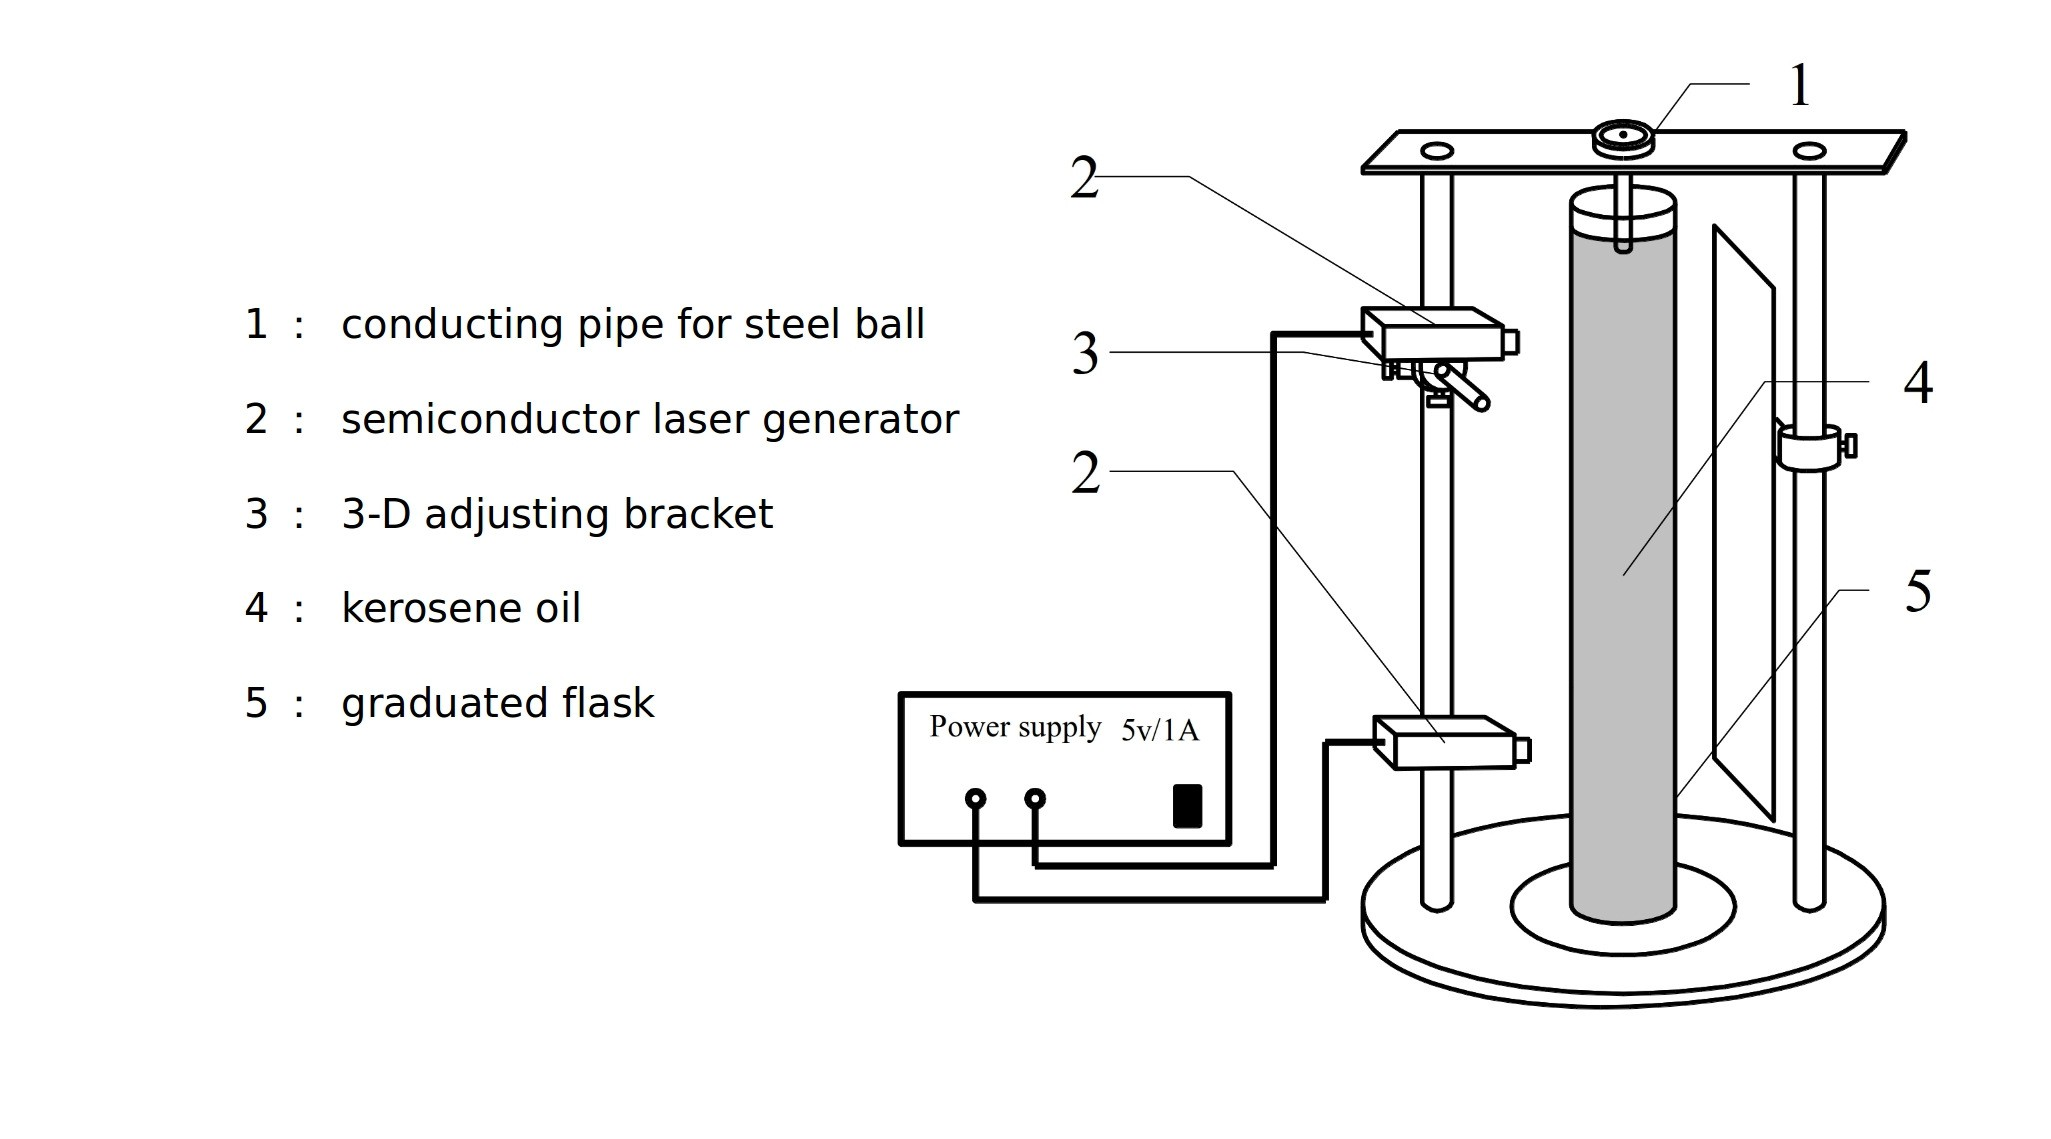
\includegraphics[width=7cm]{fig_setup.png}
	\caption{Stokes’ viscosity measurement apparatus}
	\label{fig-setup}
\end{figure}

Adjustment of the Stokes’ viscosity measurement device:
\begin{enumerate}[(1)]
	\item
	Adjust the knobs beneath the base to make the plumb aiming at the center of the base.
	\item
	Turn on the two lasers, adjust the beams so that they are parallel and aim at the plumb line.
	\item
	Remove the plumb and place the graduated flask with castor oil at the center of the base.
	\item
	Place the guiding pipe on the top of the viscosity measurement device.
	\item
	Put a metal ball into the pipe and check whether the ball, falling down in the oil, can blocks the laser beams.  If not, repeat Step 1.
\end{enumerate}

\section{Measurement}

\subsection{Measurement of the (constant) velocity of a falling ball}
\begin{enumerate}[(1)]
	\item
	Measure the vertical distance $S$ between the two laser beams at least three times.
	\item
	Put a metal ball into the guiding pipe. Start the stopwatch when the ball passes through the first beam, and stop it when it passes through the second one. Record the time $t$ and repeat the procedure for at least six times.
\end{enumerate}

\subsection{Measurement of the ball density $\bm{\rho_2}$}
\begin{enumerate}[(1)]
	\item
	Use electronic  scales  to measure the  mass of 40   metal balls. Calculate  the average to find the mass of a single ball.
	\item
	Use a micrometer to measure the diameter of the metal balls. Repeat for ten times and calculate the average  value.
	\item
	Calculate the ball density $\rho_2$.
\end{enumerate}

\subsection{Measurement of the density $\bm{\rho_1}$ of the castor oil}
\indent

Measure the density $\rho_1$ of the castor oil by using the provided densimeter (one measurement). Use a calliper to measure the inner diameter $D$ of the graduated flask for six times. Read the ambient temperature from the thermometer placed in the lab.

\subsection{Calculation of the value of viscosity coefficient $\bm{\eta}$ using Eq.(\ref{ETA3})}

\section{Results}

\subsection{Measurement of the (constant) velocity of a falling ball.}
\indent

The vertical distance $S$ between the two laser beams was calculated based on the results presented in Table.\ref{distance}.

$$\bar{S}=\frac{1}{3}\sum_{i=1}^3S_i=164.3\pm0.5mm$$

\begin{table}[!h]
\begin{center}
\begin{tabular}{cc}
\hline
\textit{Measurement} & $S$ [mm] $\pm$ 0.5 [mm] \\
\hline
1	&	164.0\\
2	&	165.0\\
3	&	164.0\\
\hline
\end{tabular}
\caption{Distance measurement data.}\label{distance}
\end{center}
\end{table}

The time $t$ through the metal ball passing through the first and second laser beam was calculated based on the results presented in Table.\ref{time}.

$$\bar{t}=\frac{1}{6}\sum_{i=1}^6t_i=9.13\pm0.41s$$

\begin{table}[!h]
\begin{center}
\begin{tabular}{cc}
\hline
\textit{Measurement} & $t$ [s] $\pm$ 0.01 [s] \\
\hline
1	&	9.12\\
2	&	8.96\\
3	&	9.26\\
4	&	9.07\\
5	&	9.00\\
6	&	9.37\\
\hline
\end{tabular}
\caption{Time measurement data.}\label{time}
\end{center}
\end{table}

\subsection{Measurement of the ball density $\bm{\rho_2}$}

The mass $m$ of 40 metal balls was measured by electronic scales
$$m=1.311\pm0.001g$$

Thus the mass of a single ball is
$$m'=\frac{m}{40}=0.032775\pm0.000025g$$

The diameter $d$ of a metal ball was calculated based on the results presented in Table.\ref{diameter}.
$$\bar{d}=\sum_{i=1}^{10}d_i=1.995\pm0.004mm$$

\begin{table}[!h]
\begin{center}
\begin{tabular}{cc}
\hline
\textit{Measurement} & $d$ [mm] $\pm$ 0.004 [mm] \\
\hline
1	&	1.980\\
2	&	1.995\\
3	&	2.000\\
4	&	1.985\\
5	&	2.000\\
6	&	1.997\\
7	&	2.000\\
8	&	1.991\\
9	&	2.000\\
10	&	1.998\\
\hline
\end{tabular}
\caption{Measurement data for the diameters of the balls.}\label{diameter}
\end{center}
\end{table}
Then the ball density $\rho_2$ can be calculated through the formula $\rho=\frac{m}{V}$

$$\rho_2=\frac{m'}{\frac{4}{3}\pi(\frac{d}{2})^3}=\frac{6m'}{\pi d^3}
=\frac{6\cdot0.03275}{3.14159\cdot0.1995^3}=7.877\pm0.048g/cm^3$$ 

\subsection{Measurement of the density $\bm{\rho_1}$ of the castor oil}

The density $\rho_1$ of the castor oil was measured by the densimeter
$$\rho_1=0.956\pm0.001g/cm^3$$

The inner diameter $D$ of the flask was calculated based on the results presented in Table.\ref{Diameter}.

$$\bar{D}=\sum_{i=1}^{6}D_i=58.93\pm0.02mm$$

\begin{table}[!h]
\begin{center}
\begin{tabular}{cc}
\hline
\textit{Measurement} & $D$ [mm] $\pm$ 0.02 [mm] \\
\hline
1	&	59.00\\
2	&	58.70\\
3	&	59.10\\
4	&	58.50\\
5	&	58.70\\
6	&	59.00\\
\hline
\end{tabular}
\caption{Measurement data for the inner diameter of the flask.}\label{Diameter}
\end{center}
\end{table}

\subsection{Calculation of the value of viscosity coefficient $\bm{\eta}$ using Eq.(\ref{ETA3})}

The temperature in the lab was measured by the temperature meter
$$T=26.5\pm1^\circ{}C$$

The acceleration due to gravity in the lab is $g=9.784m/s^2$

Then the viscosity coefficient $\eta$ can be calculated
\begin{align*}
\eta&=\frac{2}{9}R^3\frac{(\rho_2-\rho_1)gt}{s}\frac{1}{1+2.4\frac{R}{R_c}}\\
&=\frac{2}{9}\cdot0.09975^3\cdot\frac{(7.877-0.956)9.784\cdot9.13}{0.1643}\cdot\frac{1}{1+2.4\cdot\frac{0.09975}{2.9465}}\\
&=0.768\pm0.035Pa\cdot s
\end{align*}

\section{Measurement uncertainty analysis}

\subsection{Uncertainty of distance measurements}
Since the measurements of the vertical distance between the two laser beams were single measurements with type-B uncertainty of $0.5mm$, the uncertainty is $u_S=0.5mm$ 

\subsection{Uncertainty of time measurements}
For a single measurement of the time by the digital timer, its uncertainty (of
type B) is $\Delta_{tB}=\Delta_{dev}=0.01s$. In the experiment, the time is found by 
taking the average of 10 measurements. In order to estimate type-A uncertainty of the time, the standard deviation of the average value is calculated as
$$S_{\bar{t}}=\sqrt{\frac{1}{n(n-1)}\sum_{i=1}^n(t_i-\bar{t})^2}$$

Using the data from Table.\ref{time} one obtains $S_{\bar{t}}=0.16s$. Taking into account that $t_{0.95}=2.57$ for $n=6$, the Type-A uncertainty is estimated as $\Delta_{tA}=2.57\cdot0.16=0.41$

Hence the combined uncertainty
$$u_{t}=\sqrt{\Delta^2_{tA}+\Delta^2_{tB}}=\sqrt{0.41^2+0.01^2}=0.41s$$

with the relative uncertainty 4.49\%

\subsection{Uncertainty of mass measurements}
Since the measurement of the mass of 40 balls was single measurement with type-B uncertainty of $0.001g$, the uncertainty is $u_m=0.001g$

So the uncertainty of one ball is $u_{m'}=\frac{u_m}{40}=0.000025g$

\subsection{Uncertainty of diameter measurements}
Since the measurement of the diameter of the balls are single measurements with type-B uncertainty of $0.004mm$, the uncertainty is $u_d=0.004mm$

Since the measurement of the inner diameter of the flask are single measurements with type-B uncertainty of $0.02mm$, the uncertainty is $u_D=0.02mm$

\subsection{Uncertainty of density measurements}
Since the measurement of the density of the caster oil was single measurement with type-B uncertainty of $0.001g/cm^3$, the uncertainty is $u_{\rho}=0.001g/cm^3$

The density of the balls can be calculated by the equation $\frac{6m'}{\pi d^3}$, by measuring the mass and the diameter of the ball. Therefore its uncertainty $u_{\rho_2}$ is found by applying the uncertainty propagation formula

\begin{align*}
u_{\rho_2}&=\sqrt{\left(\frac{\partial\rho_2}{\partial m'}\right)^2u^2_{m'}+\left(\frac{\partial\rho_2}{\partial d}\right)^2u^2_d}
=\sqrt{\left(\frac{6}{\pi d^3}\right)^2u^2_{m'}+\left(\frac{-18m'}{\pi d^4}\right)^2u^2_d}\\
&=\sqrt{\frac{36}{3.14159^2\cdot 0.1995^6}\cdot 0.000025^2+\frac{324\cdot 0.032775^2}{3.14159^2\cdot 0.1995^8}\cdot 0.0004^2}\\
&=0.048g/cm^3
\end{align*}

Hence the density of the balls found from the measurement of the fixed mass and diameter is
$$\rho_2=7.877\pm0.048g/cm^3$$

with the relative uncertainty 0.61\%

\subsection{Uncertainty of temperature measurements}
Since the measurement of the temperature was single measurement with type-B uncertainty of $1^{\circ}C$, the uncertainty is $u_{T}=1^{\circ}C$

\subsection{Uncertainty of viscosity coefficient}
The viscosity coefficient can be calculated by Eq.(\ref{ETA3}), by measuring all of the above. Therefore its uncertainty $u_{\eta}$ is found by applying the uncertainty propagation formula

\begin{align*}
u_{\eta}&=\sqrt{
	\left(\frac{\partial\eta}{\partial R}\right)^2u^2_R+
	\left(\frac{\partial\eta}{\partial \rho_2}\right)^2u^2_{\rho_2}+
	\left(\frac{\partial\eta}{\partial \rho_1}\right)^2u^2_{\rho_1}+
	\left(\frac{\partial\eta}{\partial t}\right)^2u^2_t+
	\left(\frac{\partial\eta}{\partial s}\right)^2u^2_s+
	\left(\frac{\partial\eta}{\partial R_c}\right)^2u^2_{R_c}
}\\
&=\frac{2}{9}g\left[
	\left(\frac{2RR_c(R_c+2.4R)-2.4R^2R_c}{(R_c+2.4R)^2}\cdot\frac{(\rho_2-\rho_1)t}{s}\right)^2u^2_R+
	\left(\frac{R^2R_c}{R_c+2.4R}\cdot\frac{t}{s}\right)^2u^2_{\rho_2}+
	\left(\frac{R^2R_c}{R_c+2.4R}\cdot\frac{-t}{s}\right)^2u^2_{\rho_1}+\right.\\
&\left.
	\left(\frac{R^2R_c}{R_c+2.4R}\cdot\frac{\rho_2-\rho_1}{s}\right)^2u^2_t+
	\left(\frac{R^2R_c}{R_c+2.4R}\cdot\frac{(\rho_2-\rho_1)t}{-s^2}\right)^2u^2_s+
	\left(\frac{R^2(R_c+2.4R)-R^2R_c}{(R_c+2.4R)^2}\cdot\frac{(\rho_2-\rho_1)t}{s}\right)^2u^2_{R_c}
\right]^{\frac{1}{2}}\\
&=\frac{2}{9}\cdot 9.784\left[682.95^2\cdot(2\times10^{-6})^2+(5.114\times10^{-5})^2\cdot48^2+(5.114\times10^{-5})^2\cdot1^2+0.0388^2\cdot0.41^2+\right.\\
&\quad\left.2.154^2\cdot(5\times10^{-4})^2+0.903^2\cdot(1\times10^{-5})^2\right]^{\frac{1}{2}}\\
&=0.035
\end{align*}

Hence the viscosity coefficient found from the measurement of the fixed values is
$$\eta=0.768\pm0.035Pa\cdot s$$

with the relative uncertainty 4.56\%

\section{Conclusion}
In the experiment, we found the fluid viscosity coefficient by Stokes' method, which is a common and simple method for characterizing transparent or translucent fluids with high viscosity. We first found the time for a metal ball to travel a certain distance in the fluid and then the density of the metal ball and the fluid and the radius of the ball and the container. Finally we can calculated the viscosity coefficient $eta$ according to Eq.(\ref{ETA3})

$$\eta=0.768\pm0.035Pa\cdot s$$

On the internet, we can found that the viscosity coefficient of caster oil at $26.5^{\circ}C$ is about $0.57Pa\cdot s$, and at $23^{\circ}C$ it is about $0.77Pa\cdot s$, which is much more similar to the result of my experiment. I think it's because when I did the experiment, my position is near an air conditioner, which made there a bit cooler then where the temperature meter was set. 

One problem in the experiment is that when we recorded the time, we only used our eyes and hands to control the stopwatch, which is not accurate at all. It was also reflected on the data that the uncertainty of time is high (4.49\%). I think it can be improved by using photoelectric doors to record the time. Hence the total uncertainty may decrease from the current (4.56\%).


\section{Reference}

\begin{enumerate}[(a)]
	\item
	Qin Tian, Feng Yaming, Mateusz Krzyzosiak, VP141 Exercise 2, Measurement of Fluid Viscosity, based on materials provided by the Department of Physics, Shanghai Jiaotong University.
	\item
	Viscosity coefficient of caster oil under different temperatures\\
	(http://wenku.baidu.com/link?url=eseSMAvk6PWaIT7wvgRDFyQ-AZy2OfQXaLx5JN4ZVR\\c2fsxKJqWRplwc9z9NnrDOKOgP40YgYvdnkVp-WQqyco967cQDM-TUILtgj5MZ3d3)
\end{enumerate}

\end{document}